\documentclass[12pt, a4paper]{article}
\usepackage[margin = 1in, top=1.3in, bottom = 0.8in]{geometry}
\usepackage[english]{babel}
\usepackage[utf8]{inputenc}
\usepackage{fancyhdr}
\usepackage{amsmath}
\usepackage{bm}
\usepackage{graphicx}
\usepackage{subcaption}
\usepackage[font=small,labelfont=bf]{caption}
 
\pagestyle{fancy}
\fancyhf{}
\rhead{\small{Shaan Ul Haque(180070053)\\ Samarth Singh (180050090) \\ Niraj Mahajan (180050069)}}
\lhead{CS-663 Assignment-5 : Question 3}
\rfoot{Page 1.\thepage}
 
\begin{document}
\vspace*{-22pt}
\section{Fourier Transform of the noisy image}
The Fourier Transform of the image contained unusual peak at coordinates (266, 276) and (246, 236) which correspond to frequency pairs (-10,20) and (10, -20) respectively. The image and its Fourier Transform are shown in fig. below.
\begin{figure}[h!]
  \centering
  \begin{subfigure}[b]{0.35\linewidth}
    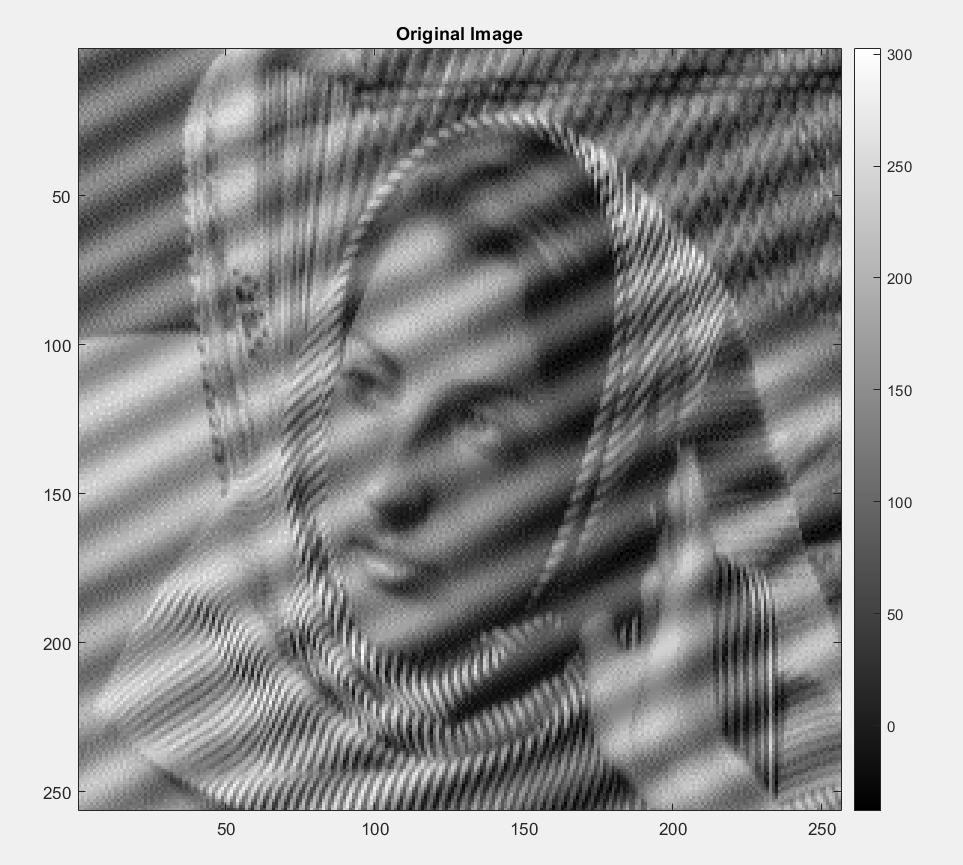
\includegraphics[width=\linewidth]{Screenshot (259).png}
    \caption{Original Image}
  \end{subfigure}
  \begin{subfigure}[b]{0.35\linewidth}
    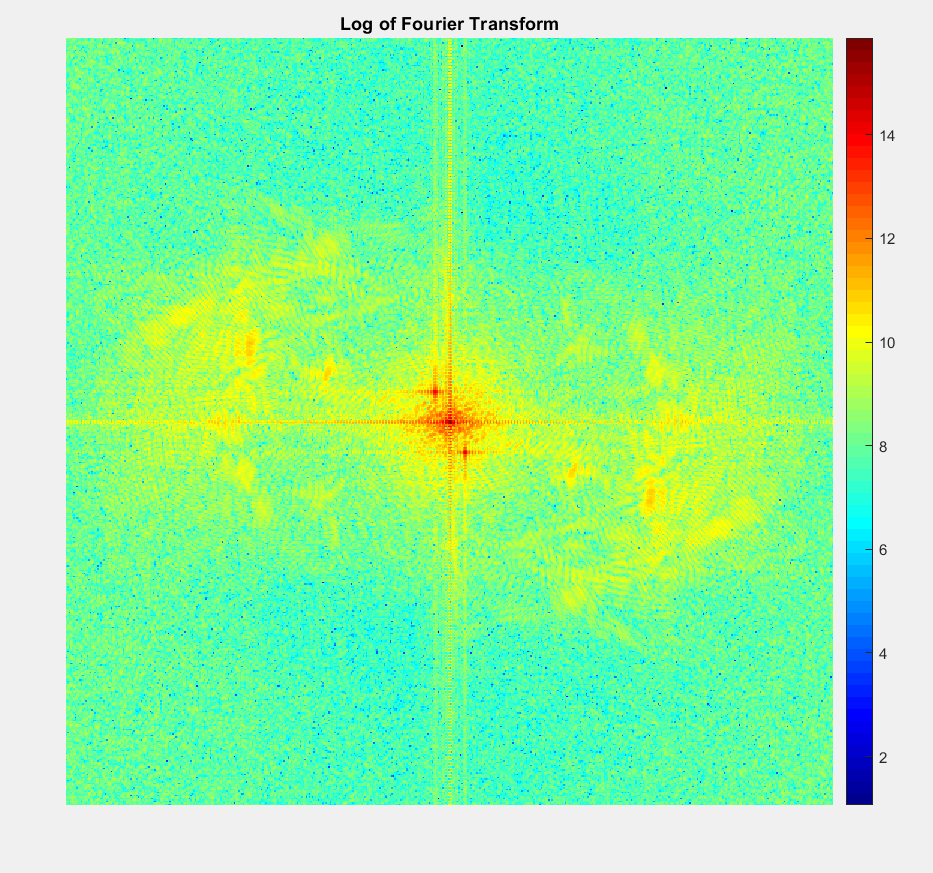
\includegraphics[width=\linewidth]{Screenshot (256).png}
    \caption{Fourier Transform}
  \end{subfigure}
  \caption{}
  \label{fig:1}
\end{figure}
This is justified also as we see the noise pattern in the image are straight lines at certain angle. The Fourier Transform of corresponding to these patterns lies on the line perpendicular to these patterns, i.e, on the line $y = -2x$. \\

To suppress this pattern we design a notch filter which is 1 everywhere in the Fourier plane but at the points nearby (266, 276) and (246, 236) where it is zero. 
\begin{equation*}
    H(u, v) = 0  \ ;\  if \ (u - u_0)^2 + (v - v_0)^2 <= D^2
\end{equation*}
\begin{equation*}
     H(u, v) = 1  ; otherwise
\end{equation*}
After some hit and trial parameter $D^2 = 14$ was found to give good results. Images are shown below. 
\begin{figure}[h!]
  \centering
  \begin{subfigure}[b]{0.35\linewidth}
    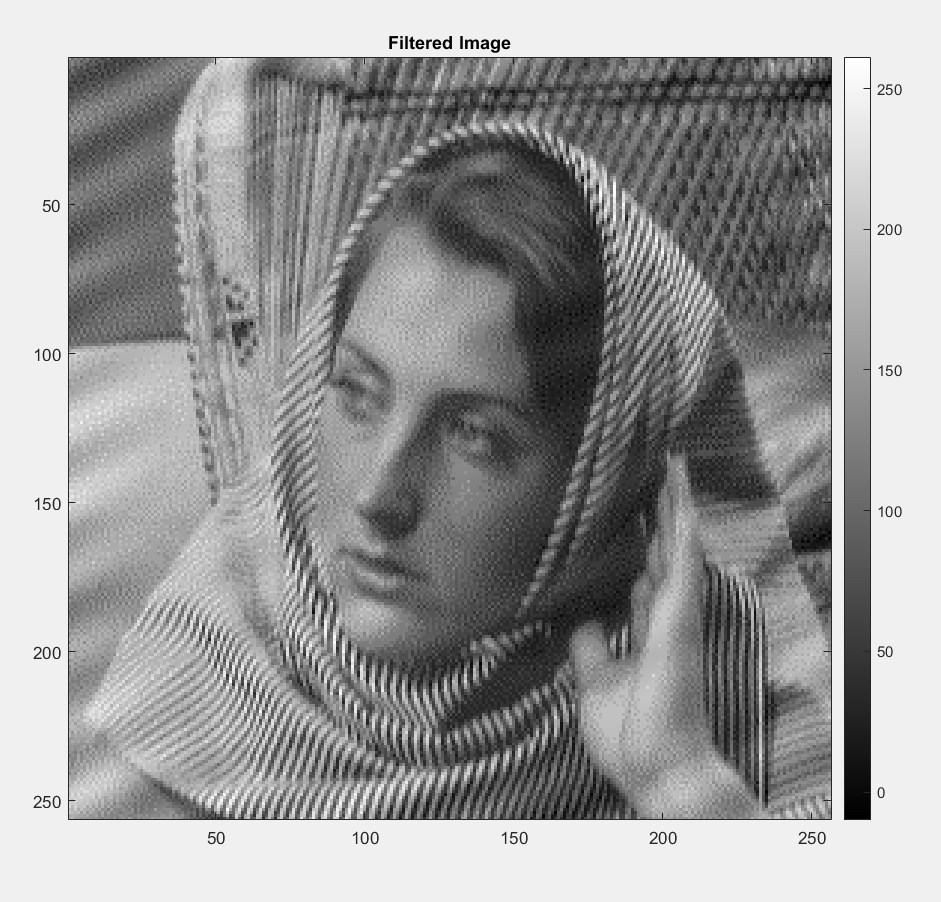
\includegraphics[width=\linewidth]{Screenshot (260).png}
    \caption{Output Image}
  \end{subfigure}
  \begin{subfigure}[b]{0.35\linewidth}
    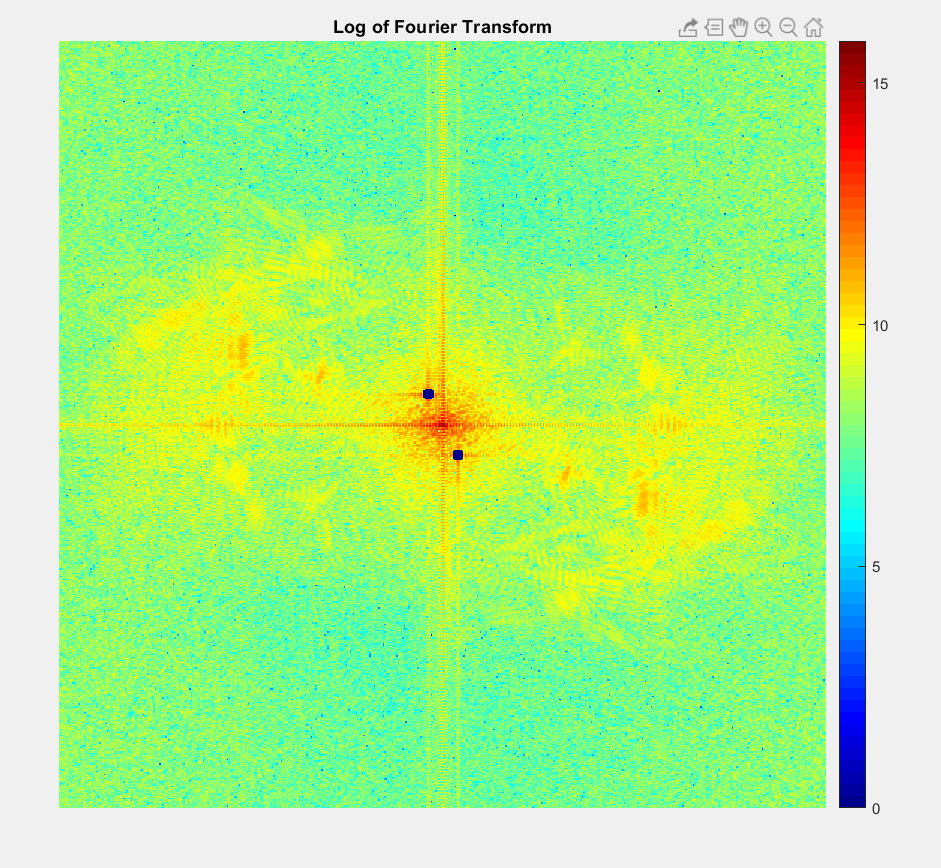
\includegraphics[width=\linewidth]{Screenshot (257).png}
    \caption{Fourier Transform}
  \end{subfigure}
  \caption{}
  \label{fig:2}
\end{figure}

\section{Code Usage}
The code is small which consists of several small parts. Firstly, we extract the image from the .mat file then display the Fourier transform (after appropriate padding) to locate the frequency corresponding to noise. The second part consists of designing notch filter in the Fourier domain, then multiplying the filter with the Fourier Transform and obtain the inverse Fourier Transform of the image. Finally we extract the middle part of the image and display it.

\end{document}
